\documentclass[twoside, final]{hcmut_report}

% Configuration
\newcommand{\var}[1]{\textbf{#1}}
\upperuniname{VIETNAM NATIONAL UNIVERSITY HO CHI MINH CITY}
\uniname{HO CHI MINH CITY UNIVERSITY OF TECHNOLOGY}
\deptname{FACULTY OF COMPUTER SCIENCE AND ENGINEERING}

\coursename{\LARGE Microcontrollers \\ \large (CO3117)}
\reporttype{\Large Report Lab 1}
\title{\Large LED ANIMATIONS}

\advisor{
TS. Lê Trọng Nhân
}
\student{
   Nguyễn Chí Thanh, 2313078
}
\setlength{\parindent}{2em}
\begin{document}
\coverpage
\pagestyle{empty}
\tableofcontents
\pagestyle{fancy}
\pagebreak
\section{Introduction}
In this lab, we will explore various LED animations using a microcontroller. The goal is to understand how to control LEDs and create visually appealing effects.
This report consists of:
\begin{itemize}
    \item Source code C language for LED animations in STM32CubeIDE.
    \item Simulate LED animations using Proteus software.
\end{itemize}
For more details about source code, visit my \href{https://batmaon512.github.io/Microcontroller-251}{GitHub repository}.
\section{Exercises}
\subsection{Exercise 1}
From the simulation on Proteus, an additional LED is connected to pin \textbf{PA6} of the STM32 microcontroller (the negative pin of the LED is connected to PA6). The recommended component for this exercise is \textbf{LED-YELLOW}, which can be found in the device list.

In this exercise, the states of the two LEDs are toggled every 2 seconds, as illustrated in the figure below.

\begin{figure}[h]
    \centering
    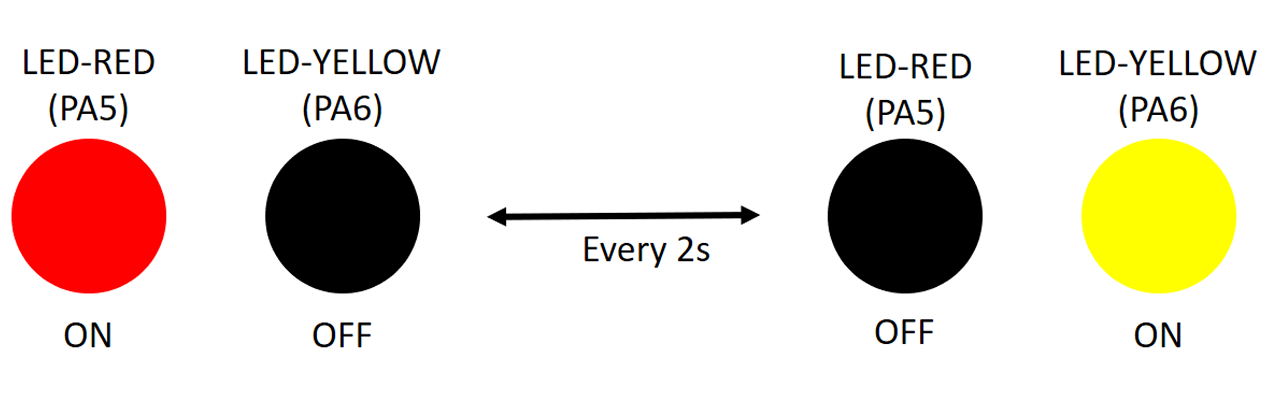
\includegraphics[width=0.7\textwidth]{graphics/f1.png}
    \caption{State transitions for 2 LEDs}
\end{figure}

\pagebreak
\textbf{Schematics from Protus simulation:}

\begin{figure}[ht]
    \centering
    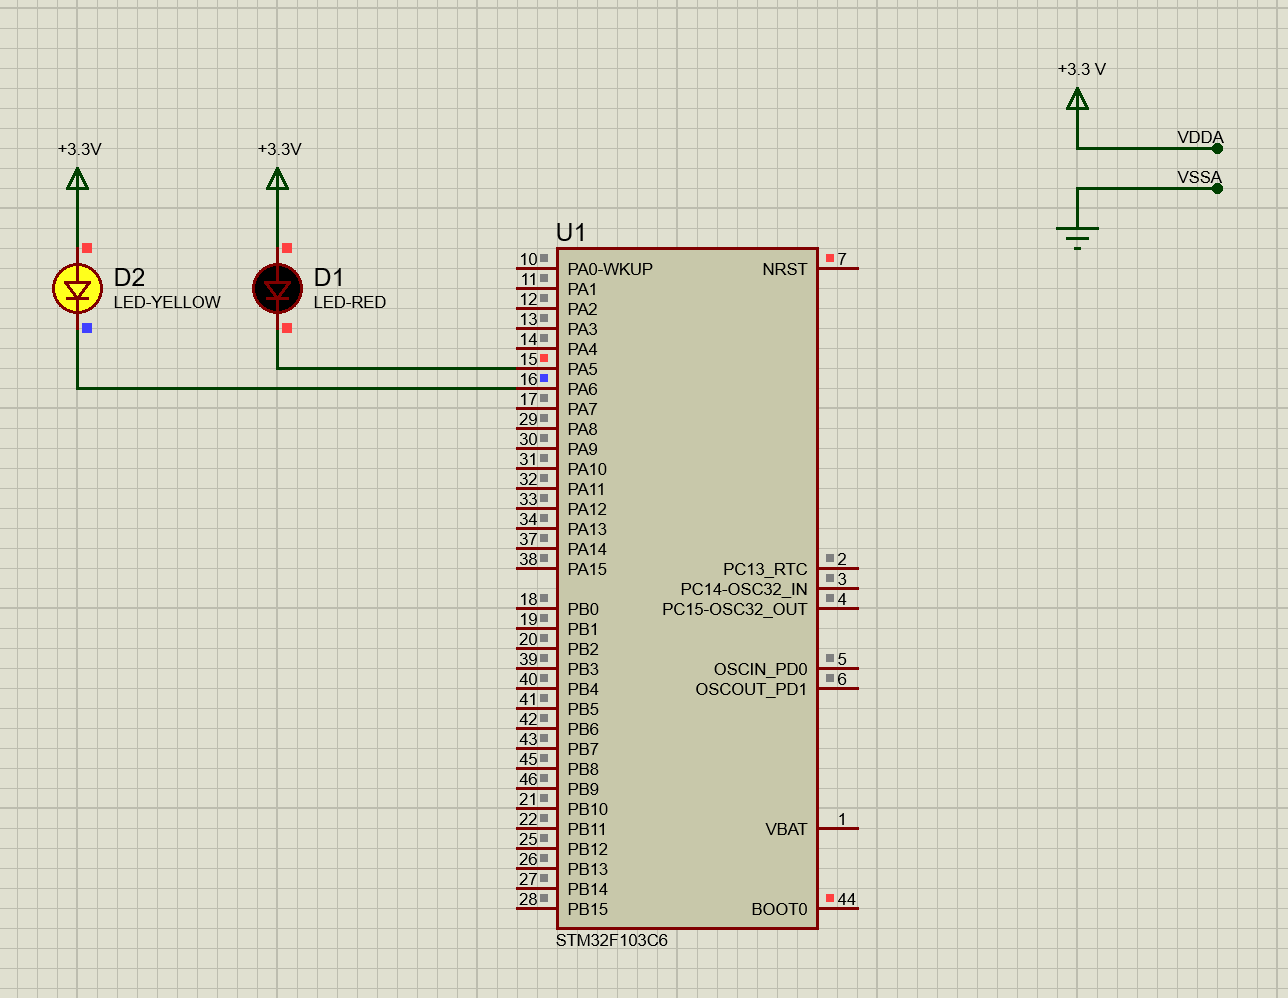
\includegraphics[width=0.6\textwidth]{graphics/f2.png}
    \caption{
        \href{https://github.com/batmaon512/Microcontroller-251/blob/main/Lab/Lab1_LED_Animations/Source_Proteus/EX1.pdsprj}{Download Proteus project file}
    }
    \label{fig:proteus_schematic}
\end{figure}

\textbf{Source code in STM32CubeIDE:}
\begin{lstlisting}[language=C, caption=Source code for Exercise 1, label=lst:ex1]
    int32_t counter = 400;
    int8_t state = -1;
    while (1){
    if(counter == 400 && state != 0){
	  		HAL_GPIO_WritePin(LED_RED_GPIO_Port, LED_RED_Pin, 1);
	  		HAL_GPIO_WritePin(LED_YELLOW_GPIO_Port, LED_YELLOW_Pin, 0);
	  		state = 0;
	}
	else if(counter == 200 && state != 1){
	  		HAL_GPIO_WritePin(LED_RED_GPIO_Port, LED_RED_Pin, 0);
	  		HAL_GPIO_WritePin(LED_YELLOW_GPIO_Port, LED_YELLOW_Pin, 1);
	  		state = 1;
	}
	else if(counter <= 1)
	  		counter = 401;
	        counter--;
	        HAL_Delay(10);
    }
\end{lstlisting}
\subsection{Exercise 2}
Extend the first exercise to simulate the behavior of a traffic light. A third LED, named \textbf{LED-GREEN} is added to the system, which is connected to pin \textbf{PA7}. A cycle in this traffic light is 5 seconds for the RED, 2 seconds for the YELLOW and 3 seconds for the GREEN. The \textbf{LED-GREEN} is also controlled by its negative pin.

Similarly, the report in this exercise includes the schematic of the circuit and the source code in the while loop.

\textbf{Schematics from Protus simulation:}

\begin{figure}[ht]
    \centering
    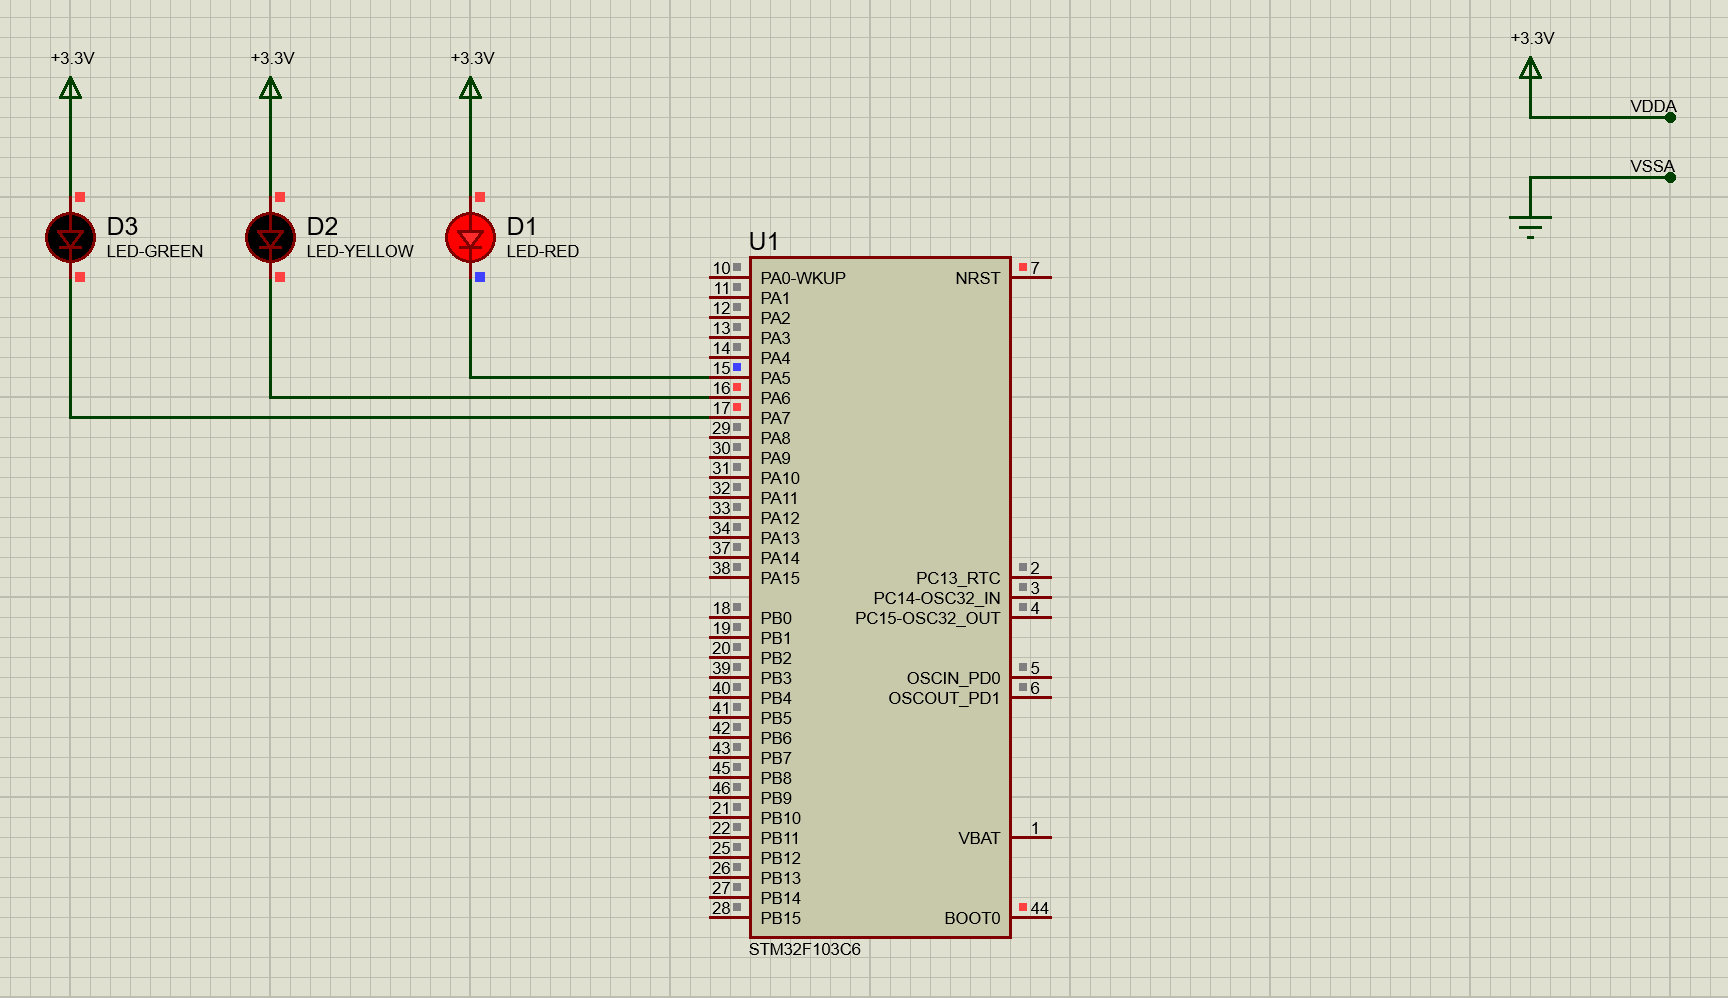
\includegraphics[width=0.7\textwidth]{graphics/f3.png}
    \caption{
        \href{https://github.com/batmaon512/Microcontroller-251/blob/main/Lab/Lab1_LED_Animations/Source_Proteus/EX2.pdsprj}{Download Proteus project file}
    }

\end{figure}

\textbf{Source code in STM32CubeIDE:}
\begin{lstlisting}[language=C, caption=Source code for Exercise 2, label=lst:ex2]
    int32_t counter = 1000;
    int8_t state = -1;
    while (1){
      if(counter == 1000 && state != 0){
	  		  HAL_GPIO_WritePin(LED_RED_GPIO_Port, LED_RED_Pin, 0);
	  		  HAL_GPIO_WritePin(LED_GREEN_GPIO_Port, LED_GREEN_Pin, 1);
	  		  HAL_GPIO_WritePin(LED_YELLOW_GPIO_Port, LED_YELLOW_Pin, 1);
	  		  state = 0;
	  }
	  else if(counter == 500 && state != 1){
	  		  HAL_GPIO_WritePin(LED_RED_GPIO_Port, LED_RED_Pin, 1);
	  		  HAL_GPIO_WritePin(LED_GREEN_GPIO_Port, LED_GREEN_Pin, 0);
	  		  HAL_GPIO_WritePin(LED_YELLOW_GPIO_Port, LED_YELLOW_Pin, 1);
	  		  state = 1;
	  }
	  else if(counter == 200 && state != 2){
  		  	  HAL_GPIO_WritePin(LED_RED_GPIO_Port, LED_RED_Pin, 1);
  		  	  HAL_GPIO_WritePin(LED_GREEN_GPIO_Port, LED_GREEN_Pin, 1);
  		  	  HAL_GPIO_WritePin(LED_YELLOW_GPIO_Port, LED_YELLOW_Pin, 0);
  		  	  state = 2;
	  }
	  else if(counter <= 1)
	  		  counter = 1001;
	  counter--;
	  HAL_Delay(10);
    }
\end{lstlisting}
\subsection{Exercise 3}
Extend to the 4-way traffic light. Arrange 12 LEDs in a nice shape to simulate the behaviors of a traffic light. A reference design can be found in the figure below.

\textbf{Schematics from Protus simulation:}

\begin{figure}[ht]
    \centering
    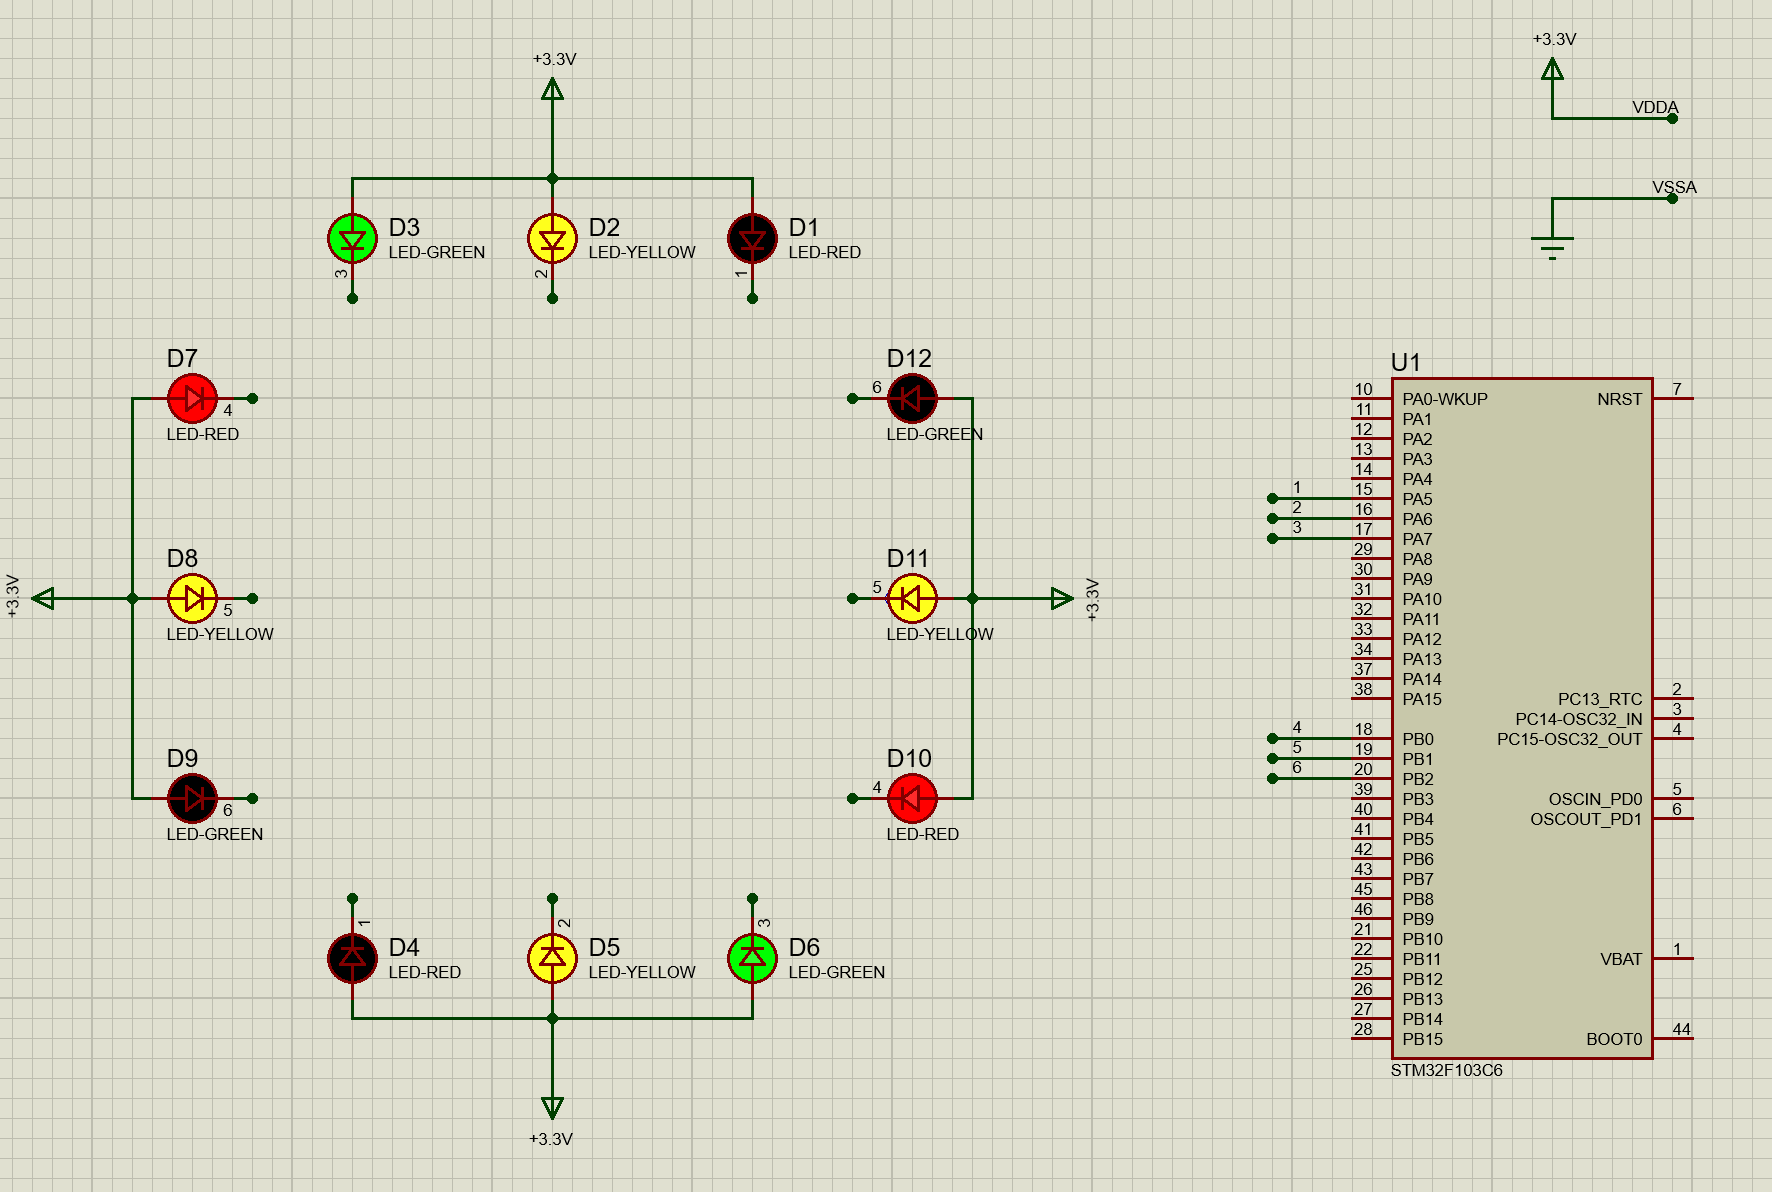
\includegraphics[width=0.7\textwidth]{graphics/f4.png}
    \caption{
        \href{https://github.com/batmaon512/Microcontroller-251/blob/main/Lab/Lab1_LED_Animations/Source_Proteus/EX3.pdsprj}{Download Proteus project file}
    }
\end{figure}
\pagebreak
\textbf{Source code in STM32CubeIDE:}
\begin{lstlisting}[language=C, caption=Source code for Exercise 3, label=lst:ex3]
//CONFIGE TIMER FOR TRAFFIC LIGHT
//NOTE: SUM OF TIME 3 LED OF TRAFFIC LIGHT MUST BE EQUAL SUM_TIME_LED
//Real Time = Time x 10 ms
//YELLOW_TIME + GREEN_TIME == RED_TIME_LED OTHER
	#define SUM_TIME_LED 1000

	#define TIME_LED_RED_1 500
	#define TIME_LED_GREEN_1 300
	#define TIME_LED_YELLOW_1 200

	#define TIME_LED_RED_2 500
	#define TIME_LED_GREEN_2 300
	#define TIME_LED_YELLOW_2 200
\end{lstlisting}

\begin{lstlisting}[language=C, caption=Source code for Exercise 3]
    int32_t counter = SUM_TIME_LED;
    int8_t state = -1;
    while(1){
        if(counter == SUM_TIME_LED && state != 0){
		  		  HAL_GPIO_WritePin(LED_RED_1_GPIO_Port, LED_RED_1_Pin, 0);
		  		  HAL_GPIO_WritePin(LED_GREEN_1_GPIO_Port, LED_GREEN_1_Pin, 1);
		  		  HAL_GPIO_WritePin(LED_YELLOW_1_GPIO_Port, LED_YELLOW_1_Pin, 1);
		  	  	  HAL_GPIO_WritePin(LED_RED_2_GPIO_Port, LED_RED_2_Pin, 1);
				  HAL_GPIO_WritePin(LED_GREEN_2_GPIO_Port, LED_GREEN_2_Pin, 0);
				  HAL_GPIO_WritePin(LED_YELLOW_2_GPIO_Port, LED_YELLOW_2_Pin, 1);
	  	  		  state = 0;
	  	  }
	  else if(counter == SUM_TIME_LED - TIME_LED_GREEN_2 && state != 1){
  		  	  	  HAL_GPIO_WritePin(LED_RED_1_GPIO_Port, LED_RED_1_Pin, 0);
  		  	  	  HAL_GPIO_WritePin(LED_GREEN_1_GPIO_Port, LED_GREEN_1_Pin, 1);
  		  	  	  HAL_GPIO_WritePin(LED_YELLOW_1_GPIO_Port, LED_YELLOW_1_Pin, 1);
  	  	  	  	  HAL_GPIO_WritePin(LED_RED_2_GPIO_Port, LED_RED_2_Pin, 1);
  	  	  	  	  HAL_GPIO_WritePin(LED_GREEN_2_GPIO_Port, LED_GREEN_2_Pin, 1);
  	  	  	  	  HAL_GPIO_WritePin(LED_YELLOW_2_GPIO_Port, LED_YELLOW_2_Pin, 0);
  	  	  	  	  state = 1;
	  }
	  else if(counter == TIME_LED_RED_2 && state != 2){
	  		  		  HAL_GPIO_WritePin(LED_RED_1_GPIO_Port, LED_RED_1_Pin, 1);
	  		  		  HAL_GPIO_WritePin(LED_GREEN_1_GPIO_Port, LED_GREEN_1_Pin, 0);
	  		  		  HAL_GPIO_WritePin(LED_YELLOW_1_GPIO_Port, LED_YELLOW_1_Pin, 1);
	  	  	  	  	  HAL_GPIO_WritePin(LED_RED_2_GPIO_Port, LED_RED_2_Pin, 0);
	  	  	  	  	  HAL_GPIO_WritePin(LED_GREEN_2_GPIO_Port, LED_GREEN_2_Pin, 1);
	  	  	  	  	  HAL_GPIO_WritePin(LED_YELLOW_2_GPIO_Port, LED_YELLOW_2_Pin, 1);
  	  		  		  state = 2;
	  	  }
	  else if(counter == TIME_LED_YELLOW_1 && state != 3){
		  		   	  HAL_GPIO_WritePin(LED_RED_1_GPIO_Port, LED_RED_1_Pin, 1);
		  		   	  HAL_GPIO_WritePin(LED_GREEN_1_GPIO_Port, LED_GREEN_1_Pin, 1);
		  		   	  HAL_GPIO_WritePin(LED_YELLOW_1_GPIO_Port, LED_YELLOW_1_Pin, 0);
	  	  	  	  	  HAL_GPIO_WritePin(LED_RED_2_GPIO_Port, LED_RED_2_Pin, 0);
	  	  	  	  	  HAL_GPIO_WritePin(LED_GREEN_2_GPIO_Port, LED_GREEN_2_Pin, 1);
	  	  	  	  	  HAL_GPIO_WritePin(LED_YELLOW_2_GPIO_Port, LED_YELLOW_2_Pin, 1);
		  		   	  state = 3;
	  	  }
	  else if(counter <= 1)
	  	  		  counter = SUM_TIME_LED+1;
	  	  counter--;
	  	  HAL_Delay(10);
    }
\end{lstlisting}
\subsection{Exercise 4}

Add \textbf{only one 7 led segment} to the schematic in Exercise 3. This component can be found in Proteus by the keyword \textbf{7SEG-COM-ANODE}. For this device, the common pin should be connected to the power supply and other pins are supposed to be connected to PB0 to PB6. Therefore, to turn-on a segment in this 7SEG, the STM32 pin should be in logic 0 (0V).

Implement a function named \textbf{display7SEG(int num)}. The input for this function is from 0 to 9 and the outputs are listed as following:


\textbf{Schematics from Protus simulation:}

\begin{figure}[ht]
    \centering
    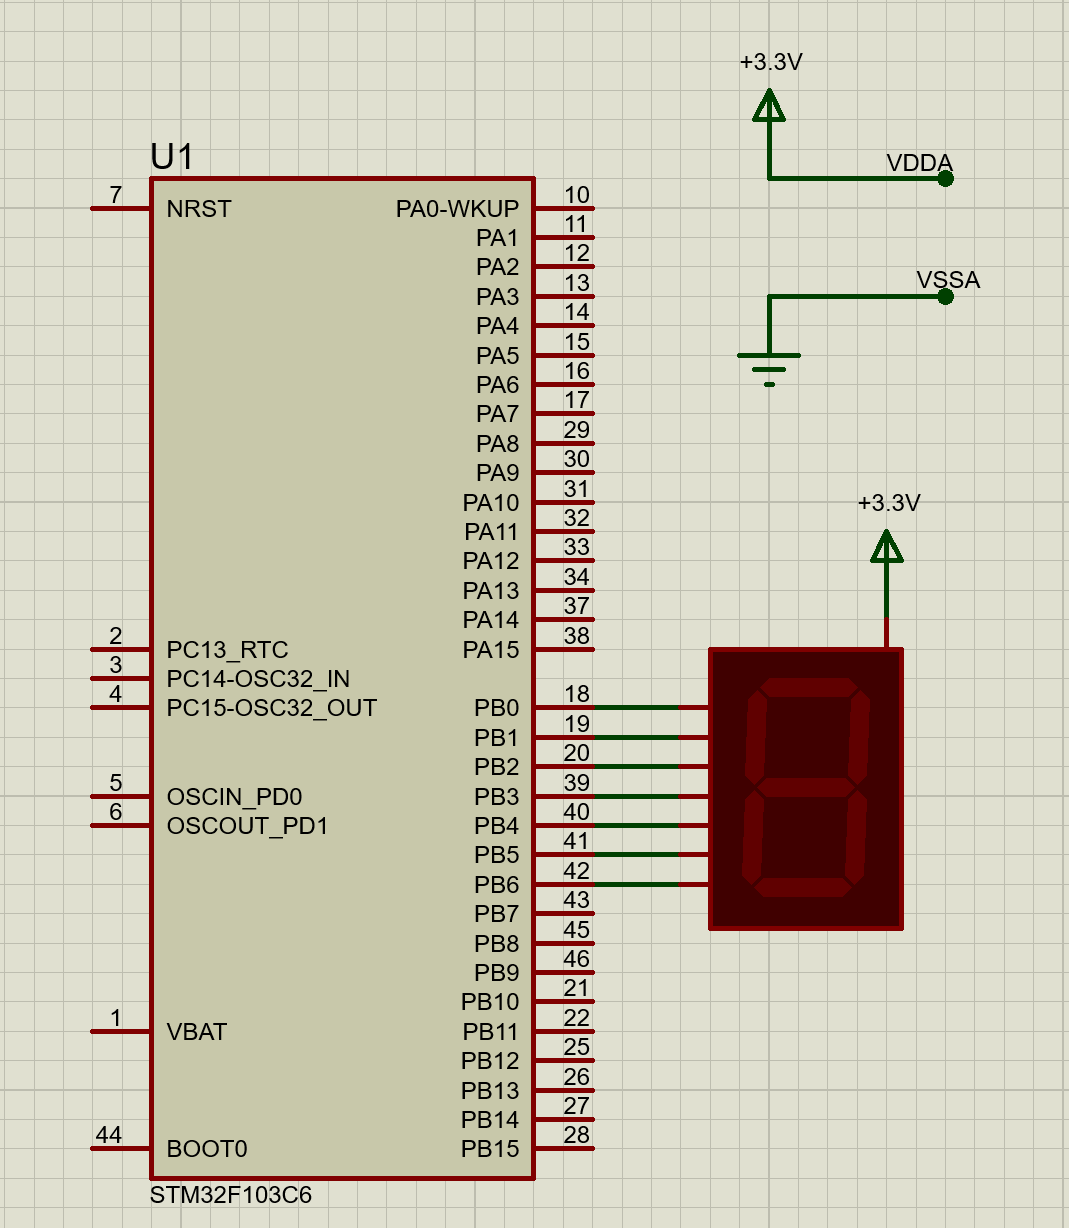
\includegraphics[width=0.5\textwidth]{graphics/f5.png}
    \caption{
        \href{https://github.com/batmaon512/Microcontroller-251/blob/main/Lab/Lab1_LED_Animations/Source_Proteus/EX4.pdsprj}{Download Proteus project file}
    }
\end{figure}
\pagebreak
\textbf{Source code in STM32CubeIDE:}
\begin{lstlisting}[language=C, caption=Source code for Exercise 4]
 void display7SEG(int counter){
	 if(counter > 9 || counter < 0) return;
	 HAL_GPIO_WritePin(PIN_A_GPIO_Port, PIN_A_Pin, counter==1 || counter==4);
	 HAL_GPIO_WritePin(PIN_B_GPIO_Port, PIN_B_Pin, counter==5 || counter==6);
	 HAL_GPIO_WritePin(PIN_C_GPIO_Port, PIN_C_Pin, counter==2);
	 HAL_GPIO_WritePin(PIN_D_GPIO_Port, PIN_D_Pin, counter==1 || counter==4 || counter==7);
	 HAL_GPIO_WritePin(PIN_E_GPIO_Port, PIN_E_Pin, !(counter == 0 || counter == 2 || counter == 6 || counter == 8));
	 HAL_GPIO_WritePin(PIN_F_GPIO_Port, PIN_F_Pin, counter==1 || counter==2 || counter==3 || counter==7);
	 HAL_GPIO_WritePin(PIN_G_GPIO_Port, PIN_G_Pin, counter== 0 || counter==1 || counter==7);
 }
\end{lstlisting}

\begin{lstlisting}[language=C, caption=Source code for Exercise 4]
    int32_t counter = 100;
	uint8_t state = 0;
    while(1){
        if(state >= 10) state = 0;
	  	if(counter <= 0){
		  	 display7SEG(state++);
		  	 counter = 100;
	  	}
	  	counter--;
	  	HAL_Delay(10);}
\end{lstlisting}

\subsection{Exercise 5}

Integrate the 7SEG-LED to the 4-way traffic light. In this case, the 7SEG-LED is used to display countdown value.

In this exercise, only source code is required to present. The function \textbf{display7SEG} in previous exercise can be re-used.

\begin{figure}[ht]
    \centering
    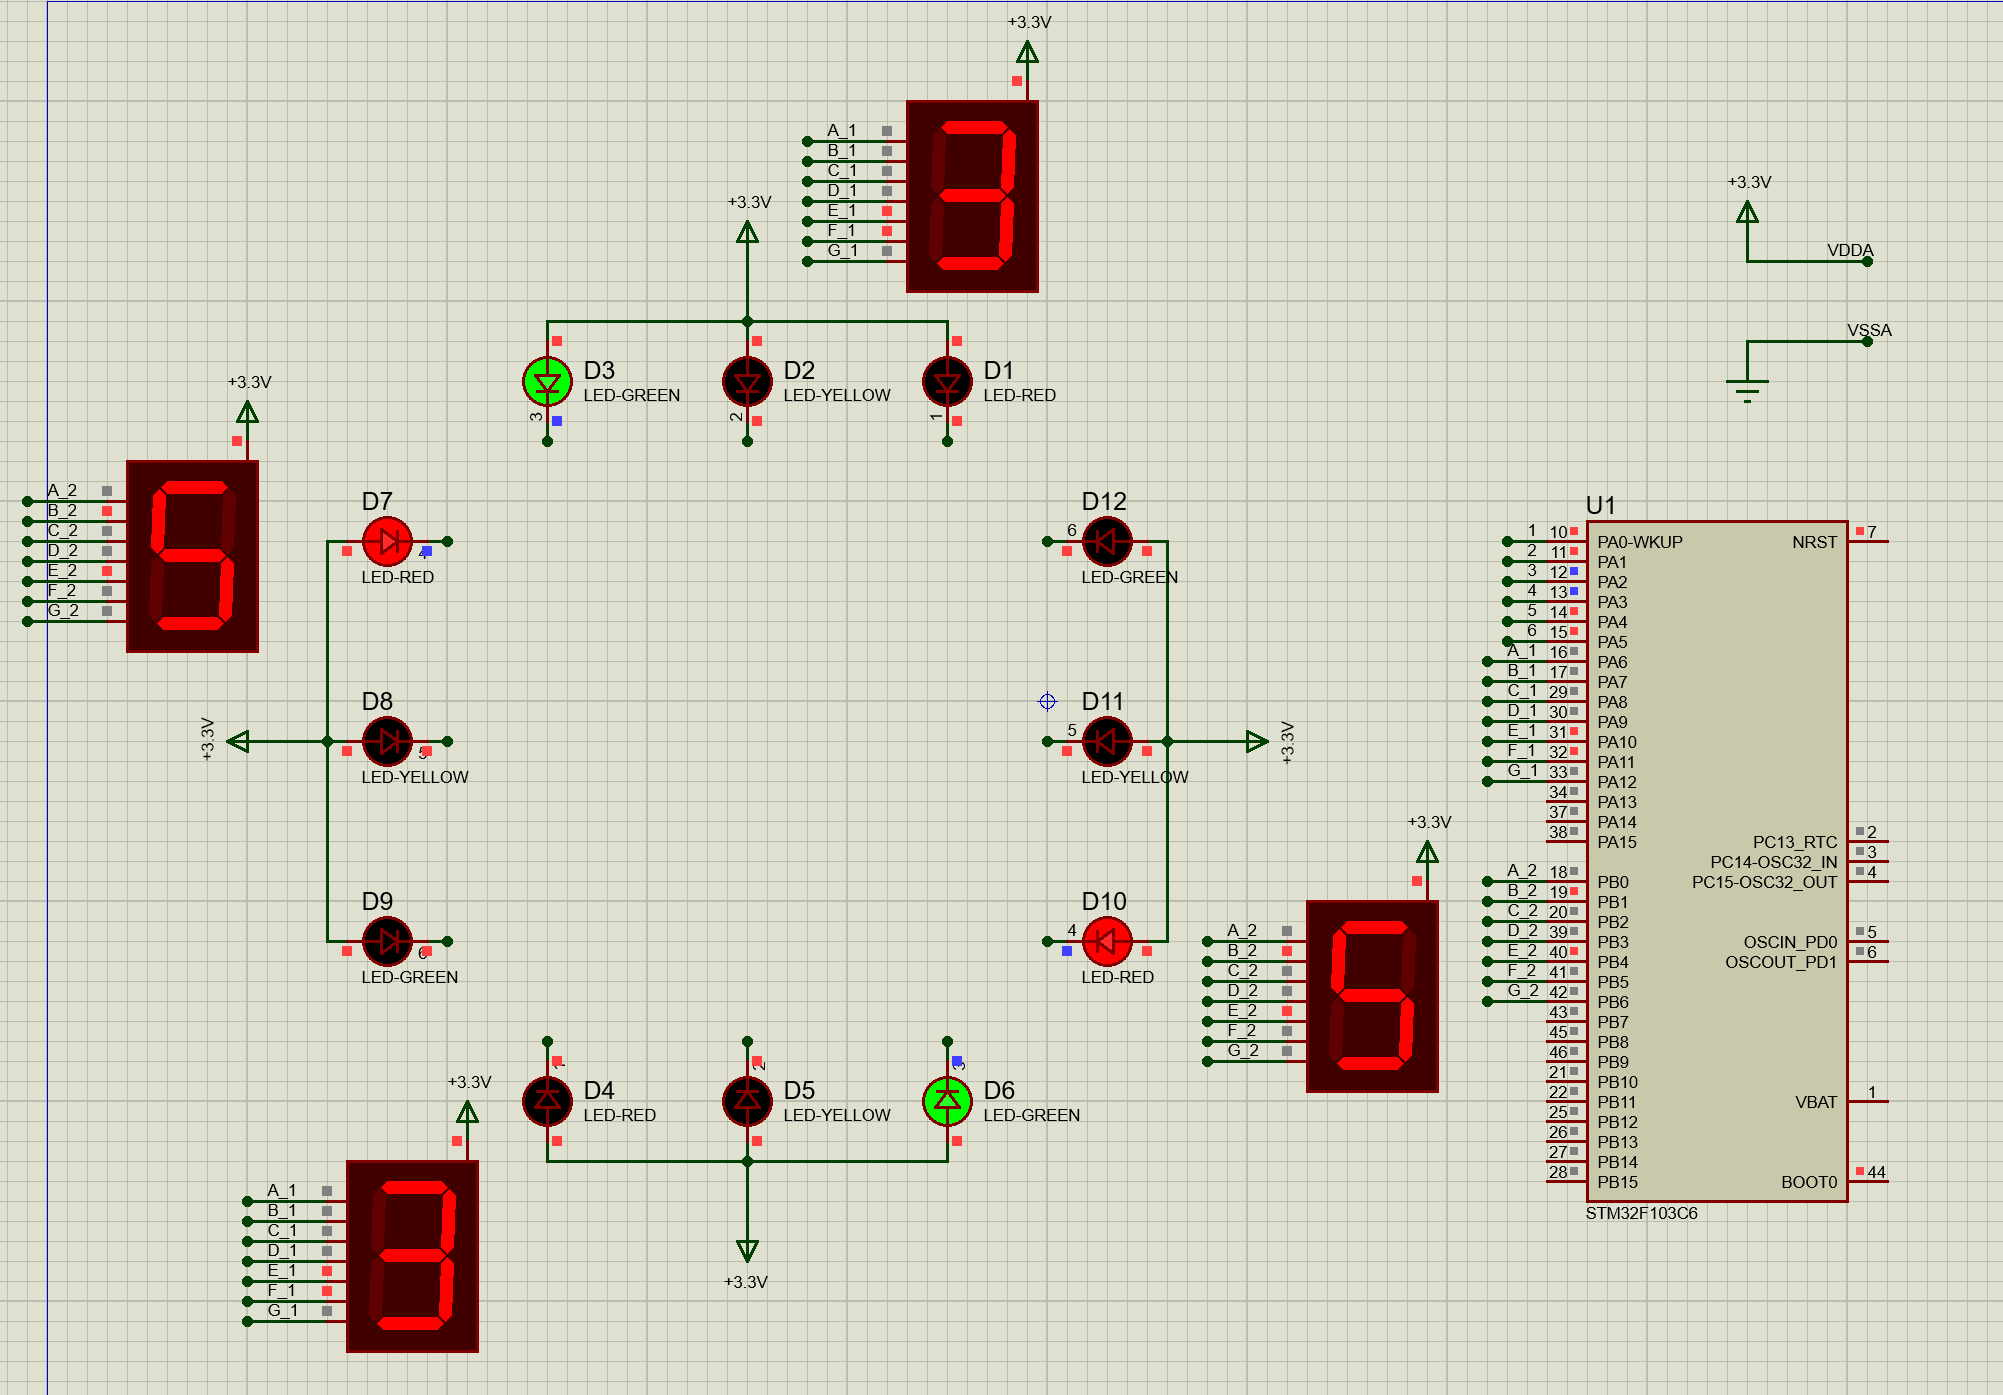
\includegraphics[width=0.7\textwidth]{graphics/f6.png}
    \caption{
        \href{https://github.com/batmaon512/Microcontroller-251/blob/main/Lab/Lab1_LED_Animations/Source_Proteus/EX5.pdsprj}{Download Proteus project file}
    }
\end{figure}

\textbf{Source code in STM32CubeIDE:}
\begin{lstlisting}[language=C, caption=Source code for Exercise 5]
 //CONFIGE TIMER FOR TRAFFIC LIGHT
 //NOTE: SUM OF TIME 3 LED OF TRAFFIC LIGHT MUST BE EQUAL SUM_TIME_LED
 //Real Time = Time x 10 ms and < 10 s
 //YELLOW_TIME + GREEN_TIME == RED_TIME_LED OTHER
#define SUM_TIME_LED 1000
#define TIME_LED_RED_1 500
#define TIME_LED_GREEN_1 300
#define TIME_LED_YELLOW_1 200
#define TIME_LED_RED_2 500
#define TIME_LED_GREEN_2 300
#define TIME_LED_YELLOW_2 200
 void display7SEG(int counter, int i){
	 if(counter > 9 || counter < 0) return;
	 if(i == 1){
	 HAL_GPIO_WritePin(PIN_A_1_GPIO_Port, PIN_A_1_Pin, counter==1 || counter==4);
	 HAL_GPIO_WritePin(PIN_B_1_GPIO_Port, PIN_B_1_Pin, counter==5 || counter==6);
	 HAL_GPIO_WritePin(PIN_C_1_GPIO_Port, PIN_C_1_Pin, counter==2);
	 HAL_GPIO_WritePin(PIN_D_1_GPIO_Port, PIN_D_1_Pin, counter==1 || counter==4 || counter==7);
	 HAL_GPIO_WritePin(PIN_E_1_GPIO_Port, PIN_E_1_Pin, !(counter == 0 || counter == 2 || counter == 6 || counter == 8));
	 HAL_GPIO_WritePin(PIN_F_1_GPIO_Port, PIN_F_1_Pin, counter==1 || counter==2 || counter==3 || counter==7);
	 HAL_GPIO_WritePin(PIN_G_1_GPIO_Port, PIN_G_1_Pin, counter== 0 || counter==1 || counter==7);
	 }
	 else{
	 HAL_GPIO_WritePin(PIN_A_2_GPIO_Port, PIN_A_2_Pin, counter==1 || counter==4);
	 HAL_GPIO_WritePin(PIN_B_2_GPIO_Port, PIN_B_2_Pin, counter==5 || counter==6);
	 HAL_GPIO_WritePin(PIN_C_2_GPIO_Port, PIN_C_2_Pin, counter==2);
	 HAL_GPIO_WritePin(PIN_D_2_GPIO_Port, PIN_D_2_Pin, counter==1 || counter==4 || counter==7);
	 HAL_GPIO_WritePin(PIN_E_2_GPIO_Port, PIN_E_2_Pin, !(counter == 0 || counter == 2 || counter == 6 || counter == 8));
	 HAL_GPIO_WritePin(PIN_F_2_GPIO_Port, PIN_F_2_Pin, counter==1 || counter==2 || counter==3 || counter==7);
	 HAL_GPIO_WritePin(PIN_G_2_GPIO_Port, PIN_G_2_Pin, counter== 0 || counter==1 || counter==7);
	 }
 }
\end{lstlisting}

\begin{lstlisting}[language=C, caption=Source code for Exercise 5]
  int32_t counter = SUM_TIME_LED;
  int8_t state = -1;
  int32_t counter_7LED = 0;
while(1){
//CONTROL LED TRAFFIC
    if(counter == SUM_TIME_LED && state != 0){
			  		  HAL_GPIO_WritePin(LED_RED_1_GPIO_Port, LED_RED_1_Pin, 0);
			  		  HAL_GPIO_WritePin(LED_GREEN_1_GPIO_Port, LED_GREEN_1_Pin, 1);
			  		  HAL_GPIO_WritePin(LED_YELLOW_1_GPIO_Port, LED_YELLOW_1_Pin, 1);
			  	  	  HAL_GPIO_WritePin(LED_RED_2_GPIO_Port, LED_RED_2_Pin, 1);
					  HAL_GPIO_WritePin(LED_GREEN_2_GPIO_Port, LED_GREEN_2_Pin, 0);
					  HAL_GPIO_WritePin(LED_YELLOW_2_GPIO_Port, LED_YELLOW_2_Pin, 1);
		  	  		  state = 0;
		  	  }
		  else if(counter == SUM_TIME_LED - TIME_LED_GREEN_2 && state != 1){
	  		  	  	  HAL_GPIO_WritePin(LED_RED_1_GPIO_Port, LED_RED_1_Pin, 0);
	  		  	  	  HAL_GPIO_WritePin(LED_GREEN_1_GPIO_Port, LED_GREEN_1_Pin, 1);
	  		  	  	  HAL_GPIO_WritePin(LED_YELLOW_1_GPIO_Port, LED_YELLOW_1_Pin, 1);
	  	  	  	  	  HAL_GPIO_WritePin(LED_RED_2_GPIO_Port, LED_RED_2_Pin, 1);
	  	  	  	  	  HAL_GPIO_WritePin(LED_GREEN_2_GPIO_Port, LED_GREEN_2_Pin, 1);
	  	  	  	  	  HAL_GPIO_WritePin(LED_YELLOW_2_GPIO_Port, LED_YELLOW_2_Pin, 0);
	  	  	  	  	  state = 1;
		  }
		  else if(counter == TIME_LED_RED_2 && state != 2){
		  		  		  HAL_GPIO_WritePin(LED_RED_1_GPIO_Port, LED_RED_1_Pin, 1);
		  		  		  HAL_GPIO_WritePin(LED_GREEN_1_GPIO_Port, LED_GREEN_1_Pin, 0);
		  		  		  HAL_GPIO_WritePin(LED_YELLOW_1_GPIO_Port, LED_YELLOW_1_Pin, 1);
		  	  	  	  	  HAL_GPIO_WritePin(LED_RED_2_GPIO_Port, LED_RED_2_Pin, 0);
		  	  	  	  	  HAL_GPIO_WritePin(LED_GREEN_2_GPIO_Port, LED_GREEN_2_Pin, 1);
		  	  	  	  	  HAL_GPIO_WritePin(LED_YELLOW_2_GPIO_Port, LED_YELLOW_2_Pin, 1);
	  	  		  		  state = 2;
		  	  }
		  else if(counter == TIME_LED_YELLOW_1 && state != 3){
			  		   	  HAL_GPIO_WritePin(LED_RED_1_GPIO_Port, LED_RED_1_Pin, 1);
			  		   	  HAL_GPIO_WritePin(LED_GREEN_1_GPIO_Port, LED_GREEN_1_Pin, 1);
			  		   	  HAL_GPIO_WritePin(LED_YELLOW_1_GPIO_Port, LED_YELLOW_1_Pin, 0);
		  	  	  	  	  HAL_GPIO_WritePin(LED_RED_2_GPIO_Port, LED_RED_2_Pin, 0);
		  	  	  	  	  HAL_GPIO_WritePin(LED_GREEN_2_GPIO_Port, LED_GREEN_2_Pin, 1);
		  	  	  	  	  HAL_GPIO_WritePin(LED_YELLOW_2_GPIO_Port, LED_YELLOW_2_Pin, 1);
			  		   	  state = 3;
		  	  }
		  else if(counter <= 1)
		  	  		  counter = SUM_TIME_LED+1;
//CONTROL 7 7SEG-LED
		  	if(counter_7LED <= 0){
		  		if(state == 0){
				  	display7SEG((TIME_LED_RED_1 - (SUM_TIME_LED - counter))/100, 1);
				  	display7SEG((TIME_LED_GREEN_2 - (SUM_TIME_LED - counter))/100, 2);
		  		}
		  		else if(state == 1){
				  	display7SEG((TIME_LED_RED_1 - (SUM_TIME_LED - counter))/100, 1);
				  	display7SEG((TIME_LED_YELLOW_2 - (SUM_TIME_LED - counter - TIME_LED_GREEN_2))/100, 2);
		  		}
		  		else if(state == 2){
				  	display7SEG((TIME_LED_GREEN_1 - (SUM_TIME_LED - counter - TIME_LED_RED_1))/100, 1);
				  	display7SEG(counter/100, 2);
		  		}
		  		else if(state == 3){
		  			display7SEG(counter/100, 1);
		  			display7SEG(counter/100, 2);
		  		}
			  	 counter_7LED = 100;
		  	}
		  	  counter_7LED--;
		  	  counter--;
		  	  HAL_Delay(10);
}
\end{lstlisting}
\subsection{Exercise 6}
In this exercise, a new Proteus schematic is designed to simulate an analog clock, with 12 different numbers. The connections for 12 LEDs are supposed to be from PA4 to PA15 of the STM32. The arrangement of 12 LEDs is depicted as follows.

\begin{figure}[h!]
    \centering
    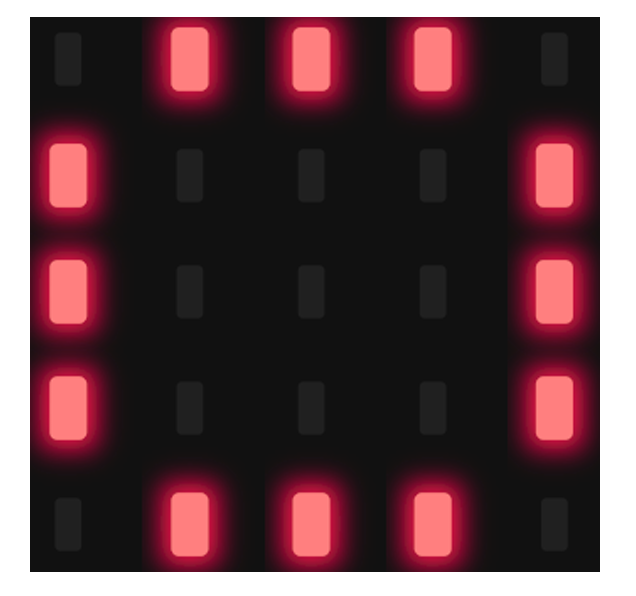
\includegraphics[width=0.3\textwidth]{graphics/f8.png}
    \caption{12 LEDs for an analog clock}
\end{figure}

\textbf{Report 1: Present the schematic.}
\begin{figure}[h!]
    \centering
    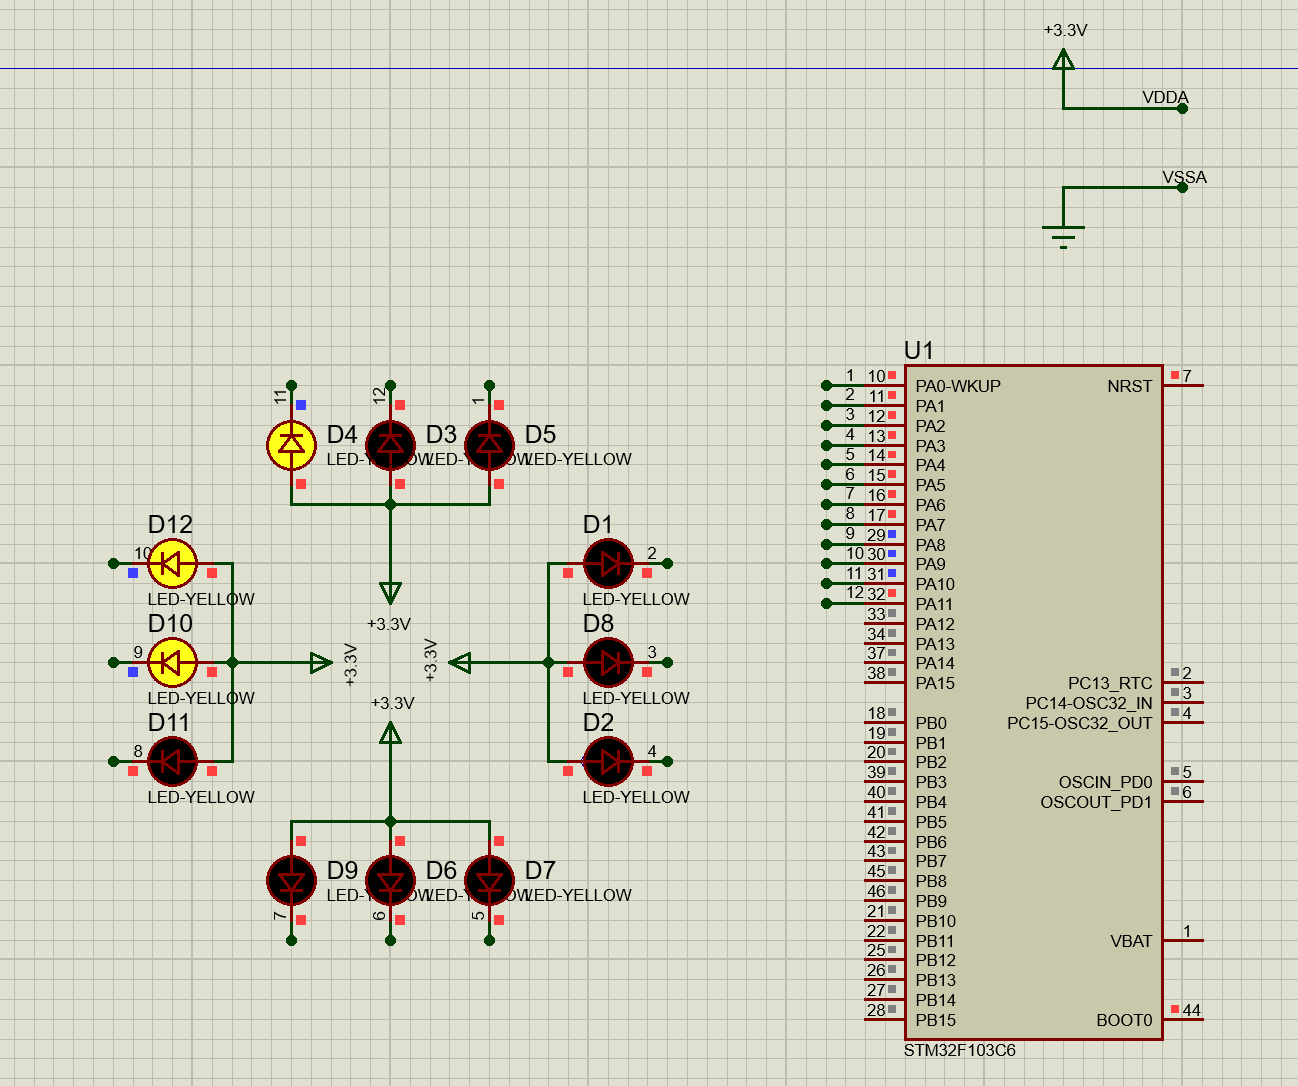
\includegraphics[width=0.7\textwidth]{graphics/f7.png}
    \caption{\href{https://github.com/batmaon512/Microcontroller-251/blob/main/Lab/Lab1_LED_Animations/Source_Proteus/EX6.pdsprj}{Download Proteus project file}}
\end{figure}

\textbf{Report 2: Implement a simple program to test the connection of every single LED. This testing program should turn every LED in a sequence.}

\begin{lstlisting}[language=C, caption=Source code for Exercise 6]
int num = 0;
int counter = 100;
while(1){
if(counter <= 0){
			  	if(num == 1){
			  		HAL_GPIO_TogglePin(PIN_1_GPIO_Port, PIN_1_Pin);
			  	}
			  	else if(num == 2){
			  		HAL_GPIO_TogglePin(PIN_2_GPIO_Port, PIN_2_Pin);
			  	}
			  	else if(num == 3){
			  		HAL_GPIO_TogglePin(PIN_3_GPIO_Port, PIN_3_Pin);
			  	}
			  	else if(num == 4){
			  		HAL_GPIO_TogglePin(PIN_4_GPIO_Port, PIN_4_Pin);
			  	}
			  	else if(num == 5){
			  		HAL_GPIO_TogglePin(PIN_5_GPIO_Port, PIN_5_Pin);
			  	}
			  	else if(num == 6){
			  		HAL_GPIO_TogglePin(PIN_6_GPIO_Port, PIN_6_Pin);
			  	}
			  	else if(num == 7){
			  		HAL_GPIO_TogglePin(PIN_7_GPIO_Port, PIN_7_Pin);
			  	}
			  	else if(num == 8){
			  		HAL_GPIO_TogglePin(PIN_8_GPIO_Port, PIN_8_Pin);
			  	}
			  	else if(num == 9){
			  		HAL_GPIO_TogglePin(PIN_9_GPIO_Port, PIN_9_Pin);
			  	}
			  	else if(num == 10){
			  		HAL_GPIO_TogglePin(PIN_10_GPIO_Port, PIN_10_Pin);
			  	}
			  	else if(num == 11){
			  		HAL_GPIO_TogglePin(PIN_11_GPIO_Port, PIN_11_Pin);
			  	}
			  	else if(num == 0){
			  		HAL_GPIO_TogglePin(PIN_12_GPIO_Port, PIN_12_Pin);
			  	}
		  		num++;
		  		if(num == 12) num = 0;
		  		counter = 50;
		  	}
		  	counter--;
		  	HAL_Delay(10);
}
\end{lstlisting}

\subsection{Exercise 7}
Implement a function named \textbf{clearAllClock()} to turn off all 12 LEDs. Present the source code of this function.

\begin{lstlisting}[language=C, caption=Source code for the clearAllClock() function]
void  clearAllClock(){
	HAL_GPIO_WritePin(PIN_1_GPIO_Port, PIN_1_Pin, 1);
	HAL_GPIO_WritePin(PIN_2_GPIO_Port, PIN_2_Pin, 1);
	HAL_GPIO_WritePin(PIN_3_GPIO_Port, PIN_3_Pin, 1);
	HAL_GPIO_WritePin(PIN_4_GPIO_Port, PIN_4_Pin, 1);
	HAL_GPIO_WritePin(PIN_5_GPIO_Port, PIN_5_Pin, 1);
	HAL_GPIO_WritePin(PIN_6_GPIO_Port, PIN_6_Pin, 1);
	HAL_GPIO_WritePin(PIN_7_GPIO_Port, PIN_7_Pin, 1);
	HAL_GPIO_WritePin(PIN_8_GPIO_Port, PIN_8_Pin, 1);
	HAL_GPIO_WritePin(PIN_9_GPIO_Port, PIN_9_Pin, 1);
	HAL_GPIO_WritePin(PIN_10_GPIO_Port, PIN_10_Pin, 1);
	HAL_GPIO_WritePin(PIN_11_GPIO_Port, PIN_11_Pin, 1);
	HAL_GPIO_WritePin(PIN_12_GPIO_Port, PIN_12_Pin, 1);
}
\end{lstlisting}
\pagebreak
\begin{lstlisting}[language=C, caption=Source code for the clearAllClock() function]
//JUST USING ONLY THIS TASK OR IF ALL PORT OF PIN 1-12 ARE SAME THIS TASK.
void clearAllClock(){
	uint16_t temp = 15;
	HAL_GPIO_WritePin(PIN_1_GPIO_Port, ~(temp<<12) , 1);
}
\end{lstlisting}

\subsection{Exercise 8}
Implement a function named \textbf{setNumberOnClock(int num)}. The input for this function is from \textbf{0 to 11} and an appropriate LED is turn on. Present the source code of this function.
\begin{lstlisting}[language=C, caption=Source code for the setNumberOnClock(int num) function]
void  setNumberOnClock(int num){
if(num > 11 || num < 0) return;
if(num == 1){
	HAL_GPIO_WritePin(PIN_1_GPIO_Port, PIN_1_Pin, 0);
}
else if(num == 2){
	HAL_GPIO_WritePin(PIN_2_GPIO_Port, PIN_2_Pin, 0);
}
else if(num == 3){
	HAL_GPIO_WritePin(PIN_3_GPIO_Port, PIN_3_Pin, 0);
}
else if(num == 4){
	HAL_GPIO_WritePin(PIN_4_GPIO_Port, PIN_4_Pin, 0);
}
else if(num == 5){
	HAL_GPIO_WritePin(PIN_5_GPIO_Port, PIN_5_Pin, 0);
}
else if(num == 6){
	HAL_GPIO_WritePin(PIN_6_GPIO_Port, PIN_6_Pin, 0);
}
else if(num == 7){
	HAL_GPIO_WritePin(PIN_7_GPIO_Port, PIN_7_Pin, 0);
}
else if(num == 8){
	HAL_GPIO_WritePin(PIN_8_GPIO_Port, PIN_8_Pin, 0);
}
else if(num == 9){
	HAL_GPIO_WritePin(PIN_9_GPIO_Port, PIN_9_Pin, 0);
}
else if(num == 10){
	HAL_GPIO_WritePin(PIN_10_GPIO_Port, PIN_10_Pin, 0);
}
else if(num == 11){
	HAL_GPIO_WritePin(PIN_11_GPIO_Port, PIN_11_Pin, 0);
}
else if(num == 0){
	HAL_GPIO_WritePin(PIN_12_GPIO_Port, PIN_12_Pin, 0);
}
}s
\end{lstlisting}

\begin{lstlisting}[language=C, caption=Source code for the setNumberOnClock(int num) function]
//JUST USING ONLY THIS TASK OR IF ALL PORT OF PIN 1-12 ARE SAME THIS TASK.
void  setNumberOnClock(int num){
if(num > 11 || num < 0) return;
HAL_GPIO_WritePin(PIN_1_GPIO_Port, 1<<num, 0);
}
\end{lstlisting}
\subsection{Exercise 9}
Implement a function named \textbf{clearNumberOnClock(int num)}. The input for this function is from \textbf{0 to 11} and an appropriate LED is turn off.
\begin{lstlisting}[language=C, caption=Source code for the clearNumberOnClock(int num) function]
void clearNumberOnClock(int num){
	if(num > 11 || num < 0) return;
	if(num == 1){
		HAL_GPIO_WritePin(PIN_1_GPIO_Port, PIN_1_Pin, 1);
	}
	else if(num == 2){
		HAL_GPIO_WritePin(PIN_2_GPIO_Port, PIN_2_Pin, 1);
	}
	else if(num == 3){
		HAL_GPIO_WritePin(PIN_3_GPIO_Port, PIN_3_Pin, 1);
	}
	else if(num == 4){
		HAL_GPIO_WritePin(PIN_4_GPIO_Port, PIN_4_Pin, 1);
	}
	else if(num == 5){
		HAL_GPIO_WritePin(PIN_5_GPIO_Port, PIN_5_Pin, 1);
	}
	else if(num == 6){
		HAL_GPIO_WritePin(PIN_6_GPIO_Port, PIN_6_Pin, 1);
	}
	else if(num == 7){
		HAL_GPIO_WritePin(PIN_7_GPIO_Port, PIN_7_Pin, 1);
	}
	else if(num == 8){
		HAL_GPIO_WritePin(PIN_8_GPIO_Port, PIN_8_Pin, 1);
	}
	else if(num == 9){
		HAL_GPIO_WritePin(PIN_9_GPIO_Port, PIN_9_Pin, 1);
	}
	else if(num == 10){
		HAL_GPIO_WritePin(PIN_10_GPIO_Port, PIN_10_Pin, 1);
	}
	else if(num == 11){
		HAL_GPIO_WritePin(PIN_11_GPIO_Port, PIN_11_Pin, 1);
	}
	else if(num == 0){
		HAL_GPIO_WritePin(PIN_12_GPIO_Port, PIN_12_Pin, 1);
	}
}
\end{lstlisting}

\begin{lstlisting}[language=C, caption=Source code for the clearNumberOnClock(int num) function]
//JUST USING ONLY THIS TASK OR IF ALL PORT OF PIN 1-12 ARE SAME THIS TASK.
void clearNumberOnClock(int num){
	if(num > 11 || num < 0) return;
	HAL_GPIO_WritePin(PIN_1_GPIO_Port, 1<<num, 1);
}
\end{lstlisting}
\subsection{Exercise 10}
Integrate the whole system and use 12 LEDs to display a clock. At a given time, there are only 3 LEDs are turn on for hour, minute and second information.

\begin{lstlisting}[language=C, caption=Source code for Exercise 10 in macro define]
#define second_init  1; //(1 - 60)
#define minute_init  49; //(1 - 60)
#define hour_init  3; //(1-12)
\end{lstlisting}
\begin{lstlisting}[language=C, caption=Source code for Exercise 10 in while loop]
  int8_t hour = hour_init;
  int8_t minute = minute_init;
  int8_t second = second_init;
  int32_t counter = 50;
  while(1){
	if(counter <= 0){
		  			  		  second++;
		  				  	  if(second > 59){
		  				  		  minute++;
		  					  	  if(minute > 59){
		  					  		  hour++;
		  						  	  if(hour > 11){
		  						  		  hour = 0;
		  						  	  }
		  					  		  minute = 0;
		  					  	  }
		  				  		  second = 0;
		  				  	  }
		  				  		  clearAllClock();
		  				  		  setNumberOnClock(second/5);
		  				  	  	  setNumberOnClock(minute/5);
		  				  	  	  setNumberOnClock(hour);
		  				  	  	  counter = 100;
		  			  	  }
		  	counter--;
		  	HAL_Delay(10);
  }
\end{lstlisting}
\pagebreak
\section*{References}
% \addcontentsline{toc}{section}{References}
% \bibliographystyle{plainnat} % Reference style
% \bibliography{references} % .bib file containing references
\end{document}